\documentclass[11pt]{article}

\usepackage{amsmath}
\usepackage{enumerate}
\usepackage{xcolor}
\usepackage{pgfplots}
\usepackage{tikz}

% Define bar chart colors
%
\definecolor{bblue}{HTML}{4F81BD}
\definecolor{rred}{HTML}{C0504D}
\definecolor{ggreen}{HTML}{9BBB59}
\definecolor{ppurple}{HTML}{9F4C7C}
\definecolor{oorange}{HTML}{FFA500}
\definecolor{yyellow}{HTML}{44DDDD}

\usepackage{titlesec}
\titlespacing*{\section}{0pt}{0.4\baselineskip}{0.2\baselineskip}

% MARGINS (DO NOT EDIT) ---------------------------------------------
\oddsidemargin  0in \evensidemargin 0in \topmargin -0.5in
\headheight 0in \headsep 0.1in
\textwidth  6.5in \textheight 9.8in
\parskip 1.25ex  \parindent 0ex \footskip 20pt
% ---------------------------------------------------------------------------------

\title{Application of Machine Learning to Link Prediction - Milestone}
\author{Kyle Julian (kjulian3), Wayne Lu (waynelu)}
\date{November 22, 2016}
\begin{document}
\maketitle
   
\section{Background and Introduction}
A real-world network is often modeled as a graph $G$ with vertices $V$ and edges $E$, denoted as $G = (V, E)$. The following terms are often used interchangeably: network/graph, node/vertex, and link/edge. Nodes represent objects in the domain such as people or products, and links represent relationships such as Facebook friendships or the purchase of a product. Links can be either directed or undirected, representing a one-way or mutual relationship, respectively. For example, Twitter follows are one-way while Facebook friendships are mutual.

Edges are notated as a pair of nodes $(u, v)$. In a directed graph, this represents an edge from $u$ to $v$. In an undirected graph, this represents a bidirectional edge between $u$ and $v$. Two nodes $u$ and $v$ are called adjacent if there exists either an edge $(u, v)$ or an edge $(v, u)$. The neighborhood of a node $u$ is the set of nodes adjacent to $u$. A node and edge are called incident if the node is one of the endpoints of the edge. The degree of a node $u$ is equal to the number of edges incident to $u$, denoted $d(u)$. For a directed graph, the in-degree of a node $u$ is equal to the number of edges pointing into $u$, denoted $d_{\text{in}}(u)$, and the out-degree of $u$ is equal to the number of edges pointing out of $u$, denoted $d_{\text{out}} (u)$.

Real-world networks evolve over time as new nodes and links are added. Link prediction algorithms use historical data in order to predict the appearance of a new links in the network or to identify links which may exist but are not represented in the data. The application of link prediction is most commonly seen in recommendation engines, either for connections on social networks or products on shopping sites. Traditional approaches involve the calculation of a heuristic score for a pair of nodes, such as the number of common neighbors or the shortest path length connecting the nodes. In this project, we will apply supervised learning algorithms to the link prediction prediction problem using a large set of topological features. The use of a large set of features allows us to then apply feature selection algorithms to identify the most important features for link prediction. Furthermore, by using only topological features and remaining domain-agnostic, we are able to investigate structural similarities between network.

\section{Related Work}
Link prediction and the application of machine learning techniques to link prediction both have significant corpuses of work behind them. Liben-Nowell and Kleinberg used a variety of topological heuristic scores as link predictors for arXiv co-authorship networks and compared their relative performances [1]. Al Hasan et al. applied supervised learning to link prediction on the BIOBASE and DBPL co-authorship networks, using both topological and domain-specific features [2]. Leskovec et al. applied supervised learning to edge sign detection in real-world social networks, notably comparing the performance of trained algorithms across different datasets and using the idea of triads as part of their feature set [3].

\section{Methodology}
\subsection{Datasets}
The data used in this project are publicly available from Stanford Network Analysis Project (SNAP). Our current datasets consist of the Wikipedia Request for Adminship (RfA) voting network and the five arXiv co-authorship networks used by Liben-Nowell and Kleinberg.

\begin{center}
    \begin{tabular}{l|r|r}
    \textbf{Dataset} & \textbf{Nodes} & \textbf{Edges} \\ \hline
    Wikipedia RfA & 7,115 & 103,689 \\ \hline
    arXiv Astro Physics & 18,722 & 198,110 \\ \hline
    arXiv Condensed Matter & 23,133 & 93,497 \\ \hline
    arXiv General Relativity & 5,242 & 14,496 \\ \hline
    arXiv High Energy Physics & 12,008 & 118,521 \\ \hline
    arXiv High Energy Physics Theory & 9,877 & 25,998
    \end{tabular}
\end{center}
\subsection{Features}
Our preliminary feature set consists of 17 topological characteristics: 8 degree features and 9 neighborhood features. Given a pair of nodes $u$ and $v$, our degree features consist of $d_{\text{in}}(u)$, $d_{\text{out}}(u)$, $d_{\text{in}}(u) / d_{\text{out}}(u)$, $d_{\text{out}}(u) / d_{\text{in}}(u)$, $d_{\text{in}}(v)$, $d_{\text{out}}(v)$, $d_{\text{in}}(v) / d_{\text{out}}(v)$, $d_{\text{out}}(v) / d_{\text{in}}(v)$. 

Our neighborhood features draw inspiration from the triads described by Leskovec et al. [3]. For a pair of nodes $u$ and $v$ and a common neighbor $w$, we identify four different triad types:
\begin{center}
\begin{tabular}{r|r}
Type 0 & $u \rightarrow w \rightarrow v$ \\ \hline
Type 1 & $u \rightarrow w \leftarrow v$ \\ \hline
Type 2 & $u \leftarrow w \rightarrow v$ \\ \hline
Type 3 & $u \leftarrow w \leftarrow v$
\end{tabular}
\end{center}
The participation rate $t_n$ of $u$ and $v$ in a Type $n$ triad is the number of common neighbors to $u$ and $v$ which form that triad. Our neighborhood features then consist of the number of common neighbors $C(u, v)$, $t_0$, $t_1$, $t_2$, $t_3$, $t_0 / C(u, v)$, $t_1 / C(u, v)$, $t_2 / C(u, v)$, and $t_3 / C(u, v)$.

\subsection{Example Generation}
For each dataset, training and testing examples were generated by first partitioning the existing edges into training and testing sets via a 90-10 split. The sets were then doubled in size by supplementing each of them with non-edge node pairs generated by random sampling. Thus, the training and testing examples contain an equal number of edge and non-edge classification examples. Finally, the previously described features were extracted for each example.

\subsection{Supervised Learning Algorithms}
We used three different classification algorithms: logistic regression, neural networks, and random forests, which are implemented in the Scikit Learn python package. The logistic regression used L2 regularization and limited-memory BFGS optimization, an efficient quasi-Newton method. The neural network classifier is comprised of 5 fully connected hidden layers of 30 nodes each with rectified linear unit activations and cross-entropy loss. The random forests algorithm trains 10 decision trees from random samples of the inputs and then averages the individual decisions to create a single decision for the forest. Because decision trees tend towards high variance, taking the average of randomized trees helps to decrease the variance and improves generalization.

\section{Preliminary Results}
First, we trained each classifier using the training data from one of the six data sets. Then, we tested the trained classifier on each data set, which tells us the generalization performance of the classifier on different data sets's testing data. The accuracies are shown in the figure below. The results show that there is a strong correlation among the graphs, especially in the co-authorship graphs. Classifiers trained on co-authorship graphs did not perform as well on the Wikipedia voting graph. However, when a neural network was trained on the Wikipedia voting graph, all of the testing sets performed well. Further work will study this correlation as well as the impact of feature selection on the classification performance.

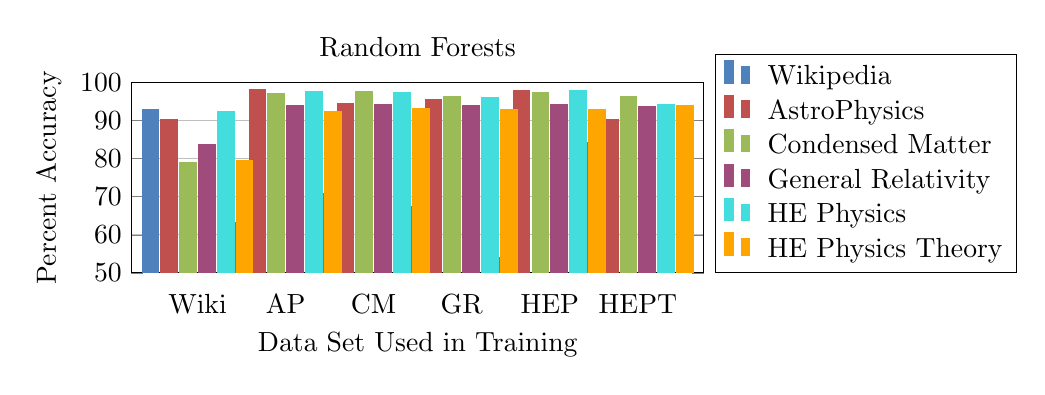
\begin{tikzpicture}
	\begin{axis}[
			width  = 0.73*\textwidth,
			height = 4cm,
			major x tick style = transparent,
			ybar=2*\pgflinewidth,
			bar width=6pt,
			ymajorgrids = true,
			ylabel = {Percent Accuracy},
			xlabel = {Data Set Used in Training},
			symbolic x coords={Wiki,AP,CM,GR, HEP, HEPT},
			xtick = data,
			ytick = {50,60,70,80,90,100},
			title = {Random Forests},
			scaled y ticks = false,
			enlarge x limits=0.15,
			ymin=50,
			ymax=100,
			legend cell align=left,
			legend style={
				at={(1.02,0)},
				anchor=south west,
				column sep=1ex
			}
		]
		\addplot[style={bblue,fill=bblue,mark=none}]
		coordinates {(Wiki, 92.78) (AP,63.228) (CM,70.91) (GR,67.342) (HEP, 54.022) (HEPT, 84.23)};
		
		\addplot[style={rred,fill=rred,mark=none}]
		coordinates {(Wiki, 90.398) (AP,98.267) (CM,94.394) (GR,95.525) (HEP, 97.796) (HEPT,90.365)};
		
		\addplot[style={ggreen,fill=ggreen,mark=none}]
		coordinates {(Wiki, 78.968) (AP,97.114) (CM,97.585) (GR,96.434) (HEP, 97.24) (HEPT,96.303)};
		
		\addplot[style={ppurple,fill=ppurple,mark=none}]
		coordinates {(Wiki, 83.661) (AP,93.858) (CM,94.168) (GR,93.841) (HEP, 94.082) (HEPT,93.72)};
		
		\addplot[style={yyellow,fill=yyellow,mark=none}]
		coordinates {(Wiki, 92.448) (AP,97.66) (CM,97.31) (GR,96.152) (HEP, 97.844) (HEPT,94.22)};
		
		\addplot[style={oorange,fill=oorange,mark=none}]
		coordinates {(Wiki, 79.43) (AP,92.409) (CM,93.198) (GR,92.804) (HEP, 92.852) (HEPT,94.054)};
		
		\legend{Wikipedia,AstroPhysics,Condensed Matter,General Relativity,HE Physics,HE Physics Theory}
	\end{axis}
\end{tikzpicture}

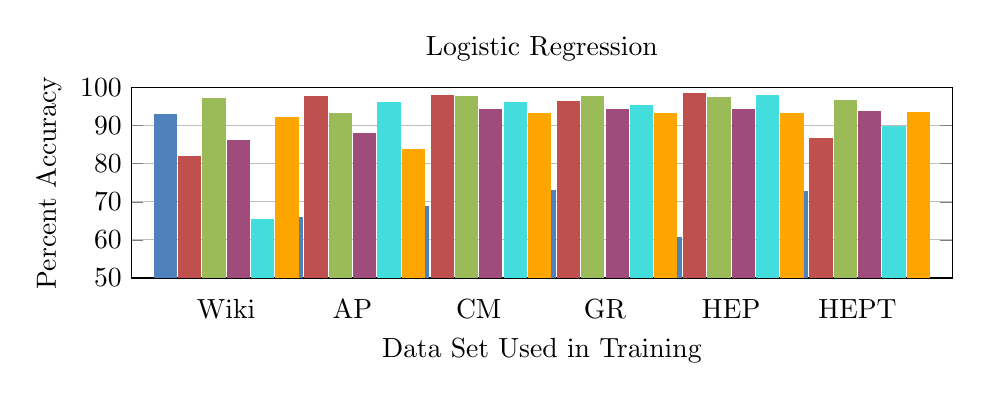
\begin{tikzpicture}
	\begin{axis}[
			width  = 0.99*\textwidth,
			height = 4cm,
			major x tick style = transparent,
			ybar=2*\pgflinewidth,
			bar width=8pt,
			ymajorgrids = true,
			ylabel = {Percent Accuracy},
			xlabel = {Data Set Used in Training},
			symbolic x coords={Wiki,AP,CM,GR, HEP, HEPT},
			xtick = data,
			ytick = {50,60,70,80,90,100},
			title = {Logistic Regression},
			scaled y ticks = false,
			enlarge x limits=0.15,
			ymin=50,
			ymax=100,
			%legend cell align=left,
			%legend style={
			%	at={(1.02,0)},
			%	anchor=south west,
			%	column sep=1ex
			%}
		]
		\addplot[style={bblue,fill=bblue,mark=none}]
		coordinates {(Wiki, 92.79) (AP,65.938) (CM,68.803) (GR,72.878) (HEP, 60.706) (HEPT, 72.801)};
		
		\addplot[style={rred,fill=rred,mark=none}]
		coordinates {(Wiki, 81.988) (AP,97.617) (CM,97.964) (GR,96.365) (HEP, 98.451) (HEPT,86.523)};
		
		\addplot[style={ggreen,fill=ggreen,mark=none}]
		coordinates {(Wiki, 97.138) (AP,93.182) (CM,97.662) (GR,97.609) (HEP, 97.435) (HEPT,96.552)};
		
		\addplot[style={ppurple,fill=ppurple,mark=none}]
		coordinates {(Wiki, 86.008) (AP,87.802) (CM,94.255) (GR,94.255) (HEP, 94.168) (HEPT,93.772)};
		
		\addplot[style={yyellow,fill=yyellow,mark=none}]
		coordinates {(Wiki, 65.345) (AP,96.108) (CM,96.179) (GR,95.350) (HEP, 97.886) (HEPT,89.705)};
		
		\addplot[style={oorange,fill=oorange,mark=none}]
		coordinates {(Wiki, 92.207) (AP,83.616) (CM,93.227) (GR,93.227) (HEP, 93.073) (HEPT,93.526)};
		
		%\legend{Wiki,AstroPhysisc,CondensedMatter,GeneralRelativity,HEPhysics,HEPhysicsTheory}
	\end{axis}
\end{tikzpicture}

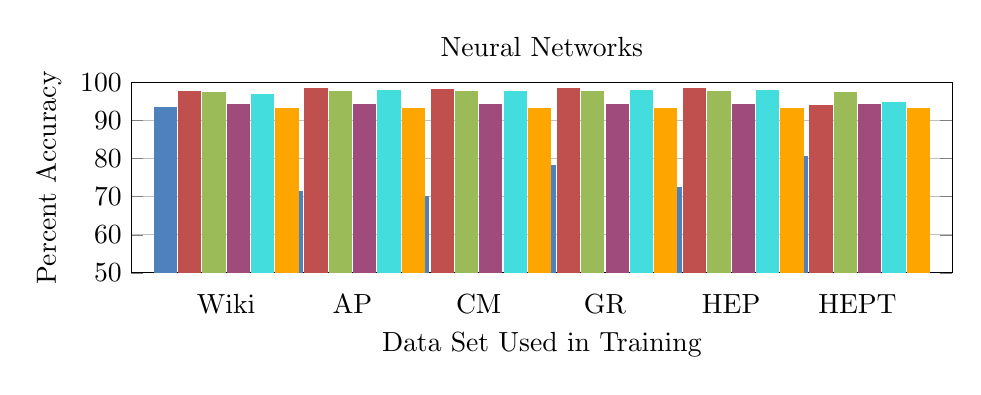
\begin{tikzpicture}
	\begin{axis}[
			width  = 0.99*\textwidth,
			height = 4cm,
			major x tick style = transparent,
			ybar=2*\pgflinewidth,
			bar width=8pt,
			ymajorgrids = true,
			ylabel = {Percent Accuracy},
			xlabel = {Data Set Used in Training},
			symbolic x coords={Wiki,AP,CM,GR, HEP, HEPT},
			xtick = data,
			ytick = {50,60,70,80,90,100},
			title = {Neural Networks},
			scaled y ticks = false,
			enlarge x limits=0.15,
			ymin=50,
			ymax=100,
			%legend cell align=left,
			%legend style={
			%	at={(1.02,0)},
			%	anchor=south west,
			%	column sep=1ex
			%}
		]
		\addplot[style={bblue,fill=bblue,mark=none}]
		coordinates {(Wiki, 93.408) (AP,71.450) (CM,70.018) (GR,78.188) (HEP, 72.323) (HEPT, 80.580)};
		
		\addplot[style={rred,fill=rred,mark=none}]
		coordinates {(Wiki, 97.586) (AP,98.482) (CM,98.172) (GR,98.295) (HEP, 98.465) (HEPT,94.069)};
		
		\addplot[style={ggreen,fill=ggreen,mark=none}]
		coordinates {(Wiki, 97.288) (AP,97.491) (CM,97.676) (GR,97.657) (HEP, 97.531) (HEPT,97.486)};
		
		\addplot[style={ppurple,fill=ppurple,mark=none}]
		coordinates {(Wiki, 94.117) (AP,94.186) (CM,94.255) (GR,94.255) (HEP, 94.220) (HEPT,94.203)};
		
		\addplot[style={yyellow,fill=yyellow,mark=none}]
		coordinates {(Wiki, 96.760) (AP,97.945) (CM,97.671) (GR,97.907) (HEP, 97.966) (HEPT,94.768)};
		
		\addplot[style={oorange,fill=oorange,mark=none}]
		coordinates {(Wiki, 93.063) (AP,93.102) (CM,93.227) (GR,93.227) (HEP, 93.160) (HEPT,93.217)};
		
		%\legend{Wiki,AstroPhysisc,CondensedMatter,GeneralRelativity,HEPhysics,HEPhysicsTheory}
	\end{axis}
\end{tikzpicture}

\section{Works Cited}
\begin{enumerate}[1.]
\item Liben-Nowell, David, and Jon Kleinberg. "The link-prediction problem for social networks." \textit{Journal of the American society for information science and technology} 58.7 (2007): 1019-1031.
\item Al Hasan, Mohammad, et al. "Link prediction using supervised learning." \textit{SDM06: workshop on link analysis, counter-terrorism and security}. 2006.
\item Leskovec, Jure, Daniel Huttenlocher, and Jon Kleinberg. "Predicting positive and negative links in online social networks." \textit{Proceedings of the 19th international conference on World wide web. ACM}, 2010.
\end{enumerate}

\end{document}